\subsection{KNN}
En esta sección definimos:
\begin{itemize}
	\item $k$: cantidad de vecinos a considerar en el algoritmo $kNN$.
\end{itemize}
El análisis sobre el algoritmo $KNN$ ($k$ vecinos más cercanos) se realiza para distintos valores de $k$, la idea detrás de esta elección, busca entender la variación en la efectividad (cantidad de aciertos) del algoritmo.
\\
Para ello variamos $k$ desde $1$ hasta $30$ para ver cual era el comportamiento que se obtenía. Para cada uno de los $k$s realizamos una corrida cross-validation con $10$ conjuntos.
\\
% El procedimiento de este algoritmo comienza, por cada imágen que queremos averiguar a que dígito pertenece, con su vectorización. Luego resta el resultado a cada uno de los vectores imágen y calcula la norma 2 para saber en cuánto difieren con cada una de las imágenes.
% Todos esos resultados se acumulan en una cola de prioridad que los ordena de menor a mayor, según las diferencias entre la imágen la cual se quiere averiguar a que clase pertenece y todas las imágenes de la base de datos etiquetada.
% \\
% Como siguiente paso se toman los $k$ primeros elementos de la cola de prioridad y se verifica a que dígito se corresponden para luego saber cuál es el dígito que recibió más "votos" y ver si se produjo un acierto o no.
% \subsubsection{Cantidad de vecinos}
% Como ya dijimos, para analizar cuál es el mejor número de vecinos para el cual el algoritmo $KNN$  da una mayor cantidad de aciertos, optamos por variar la cantidad de $k$ vecinos a tomar.
%Se prueba entonces el algoritmo $KNN$ para los siguientes valores de $k$: $1,2,3,4,...,30$.
%\\
Cada uno de los conjuntos contaba con 4200 imagenes a testear, en los siguientes graficos presentamos algunos de los sets obtenidos:

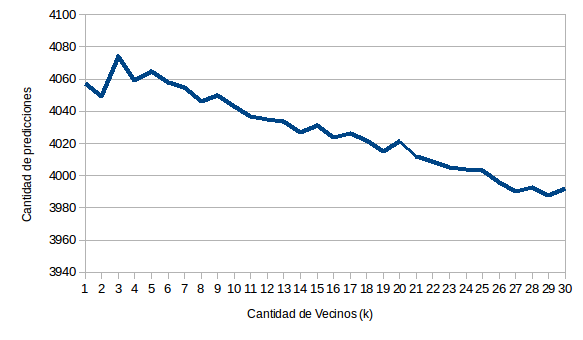
\includegraphics[scale=0.55]{nuevosResultados/knn/1.png}\\

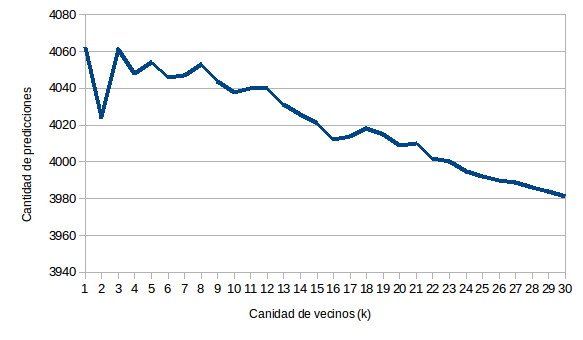
\includegraphics[scale=0.55]{nuevosResultados/knn/2.png}\\

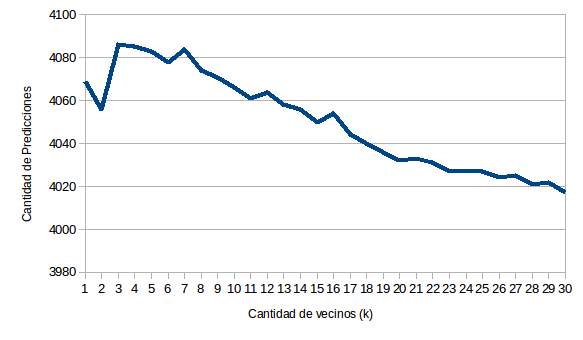
\includegraphics[scale=0.55]{nuevosResultados/knn/3.png}\\

Como puede verse hay un patrón bastante claro en los tres test corridos, para valores muy pequeños de k (k=1,K=2) podemos observar que los resultados son peores que para $k=3$,luego para valores más grandes se observa lo que nos decía la intuición, tal que para un gran número de vecinos se empiezan a perder aquellos que son realmente relevantes y las predicciones empiezan a ser peores, lo que no se esperaba era el salto en la cantidad de aciertos que vemos en los primeros valores de $k$ pero podemos entonces saber que dentro de los primeros $k$ se encuentran los mejores resultados.  
\\
Ademas para estos tests realizamos una medición de tiempos para ver cómo se comportaba el algoritmo frente a un cambio en la cantidad de vecinos. Los valores promediados para cada $k$ pueden verse en el siguiente gráfico:

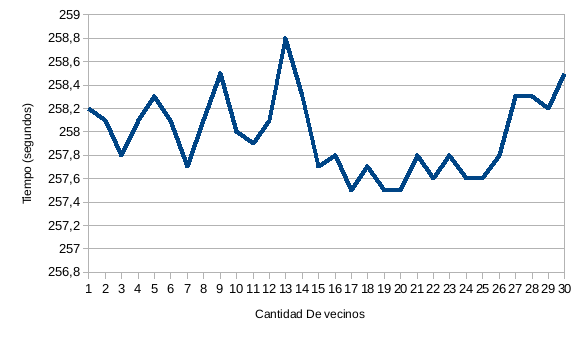
\includegraphics[scale=0.55]{nuevosResultados/knn/knntemp.png}\\

Como puede observarse, los tiempos de los algoritmos no se ven muy afectados por la variación en la cantidad de vecinos. Es muy probable que esto se deba a que el algoritmo debe comparar a la imagen que se desea comparar contra un número muy extenso de imagenes que estan en el mismo orden de magnitud. 
\completar

Luego de los test decidimos que vamos a usar $k=3$ porque nos dio los mejores resultados, cantidad de aciertos.

\subsection{PCA}
\subsubsection{Busqueda del mejor valor de $\alpha$}
En esta sección definimos:
\begin{itemize}
	\item $\alpha$: a la cantidad de componentes principales a tomar para el $PCA$.
	\item $k$: cantidad de vecinos a considerar en el algoritmo $kNN$.
\end{itemize}
En primera instancia vamos a utilizar cross-validation para intentar determinar el mejor $\alpha$ posible. Supondremos en este momento que el mejor $k$ para este caso es el encontrado en la sección anterior (aunque esto podría no ser así) y luego testeamos si esto es así o si para el $\alpha$ encontrado existe algun otro $k$ que mejora la cantidad de predicciones del sistema.
\\
Por lo tanto enfocamos nuestro análisis en obtener un valor óptimo de $\alpha$. Para este fin, partimos el conjunto de datos de entrenamiento en 10 subconjuntos y aplicamos cross-validation. Dado que este parámetro representa la cantidad de componentes principales a tener en cuenta y teniendo en mente el funcionamiento del algoritmo de PCA, es esperable que valores pequeños no sean beneficiosos (teniendo en cuenta que el máximo a considerar es bastante elevado), pero dado que PCA las ordena en base a su relevancia, se alcance un valor óptimo sin necesidad de considerarlas todas. Para esta partición de los datos de entrenamiento con 4200 imagenes para testear, tomamos $\alpha$ desde $1$ hasta $50$ y graficamos lo obtenido:

\begin{center}
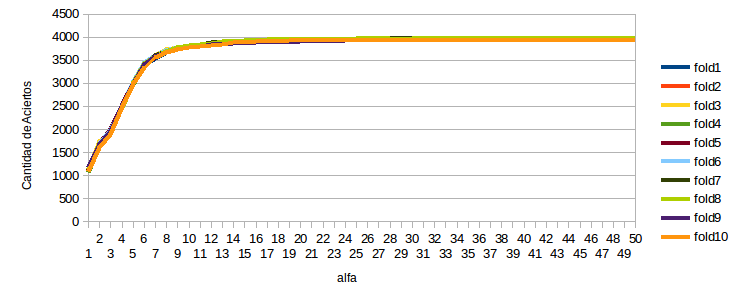
\includegraphics[scale=0.5]{nuevosResultados/pca/alfa/1.png}
\end{center}

Puede verse que para valores pequeños, aumentar en uno el $\alpha$ produce un gran aumento de aciertos. Por ejemplo, considerando el primer set para $\alpha$ igual a $1$ se obtienen $1112$ aciertos, mientras que para $\alpha$ igual a $2$ se obtienen $1680$ aciertos, esto es un $52\%$ mas de aciertos.
\\
Para valores mas grandes de $\alpha$ (alrededor de $\alpha = 12$) esta tendencia empieza estabilizarse. Por ejemplo para $\alpha = 12$ se obtienen $3845$ imagenes correctamente predecidas, pero para $\alpha = 13$ se obtienen $3869$ imagenes correctas, esto es el crecimiento de aciertos es de menos de un $1\%$.
\\
Ademas, para este k-fold medimos los tiempos de ejecución y los promediamos para poder ver de que manera varía la ejecución de los algoritmos en función de $\alpha$:

\begin{center}
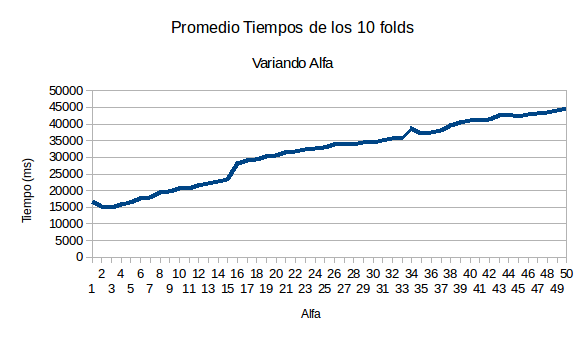
\includegraphics[scale=0.5]{nuevosResultados/pca/alfa/temp.png}
\end{center}


Cabe aclarar que estos tiempos no contemplan todo lo que se considera el 'entrenamiento' del sistema, osea, todo el preprocesamiento que resultará en encontrar los valores principales. La justificación de esto es que esto se realizará una vez, para entrenar el sistema, luego, al momento de clasificar las nuevas imagenes este tiempo podrá ser despreciado.
\\
En este grafico se puede ver que aumentar el $\alpha$ produce un aumento lineal de los tiempos de ejecución, de lo que se desprende que aumentar la cantidad valores principales no resulta gratuito y tiene cierto costo asociado.
\\
Ademas aumentar de manera desmedida el $\alpha$ puede provocar lo que en machine learning se denomina 'Overfitting'.
\inventarReferencia
\\
Debido a todas las razones expuestas consideramos que con $\alpha$ igual a $14$ será el mejor valor que podemos tomar.
\\
%falta retestear esto de abajo
\subsubsection{Busqueda del mejor valor de $k$}

La segunda prueba a realizar es, fijando un valor de $\alpha$, analizar para que cantidad de vecinos se obtiene la mayor cantidad de aciertos.
\\
Para esto tomamos $\alpha = 14$ volvemos a dividir el conjunto de datos en $10$ sets y realizamos cross validation sobre estos, variando el $k$ desde 1 hasta $30$.
\\
Los resultados obtenidos son los siguientes:
\begin{center}
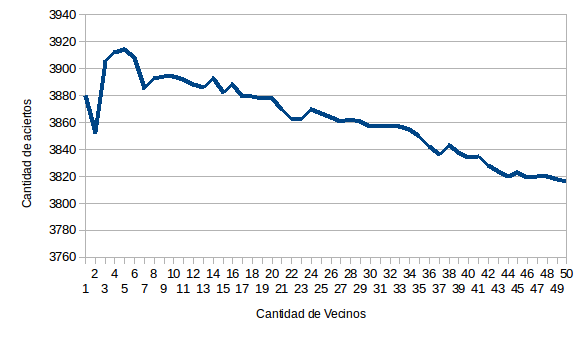
\includegraphics[scale=0.5]{nuevosResultados/pca/k/1.png}\\
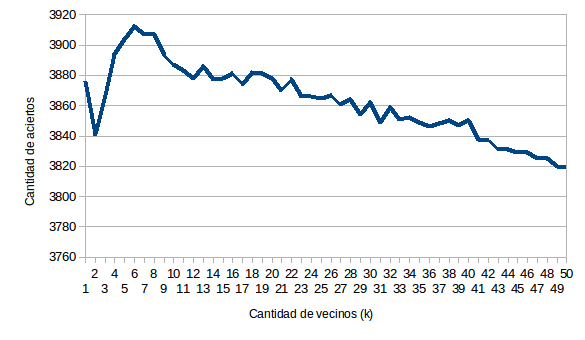
\includegraphics[scale=0.5]{nuevosResultados/pca/k/2.png}\\
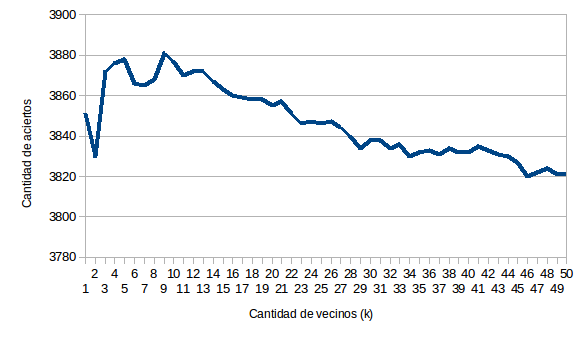
\includegraphics[scale=0.5]{nuevosResultados/pca/k/3.png}\\
\end{center}

Ademas medimos los tiempos y los promediamos para obtener una idea de cómo afectan las variaciones de $k$ a este método:
\begin{center}
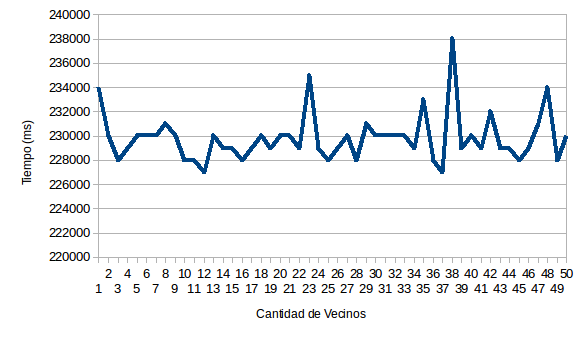
\includegraphics[scale=0.5]{nuevosResultados/pca/k/temp.png}\\
\end{center}




